%% By Nathan Burwig
%% Fall 2022 (probably)
%% This outlines the packages I use
\documentclass[11pt]{article}
\pagestyle{plain}
\usepackage[text={6.5in,9.5in},centering]{geometry}
\usepackage{amsmath}
\usepackage{graphicx}
\usepackage{caption}
\usepackage{float}
\usepackage{xcolor}
\usepackage{subcaption}

%% Defines the use of [r] on the bmatrix
\makeatletter
\renewcommand*\env@matrix[1][c]{\hskip -\arraycolsep
  \let\@ifnextchar\new@ifnextchar
  \array{*\c@MaxMatrixCols #1}}
\makeatother

\counterwithin{equation}{enumi}
\begin{document}

\noindent Nathan Burwig \\
Math 87 HW 3 \\
Due 09/28/2022 

\hrulefill

\begin{enumerate}


%%%%%%%%%%%%%%%%%%%%%%%%%%%%%%%%%%%%%%%%%%%%%%%%%%%%%%%%%%%%%%%%%%%%%%%
% Problem 1
%%%%%%%%%%%%%%%%%%%%%%%%%%%%%%%%%%%%%%%%%%%%%%%%%%%%%%%%%%%%%%%%%%%%%%%

\item \textbf{Hope for the best...}
    You have a barrel which can store seven gallons of food, and you decide
    to fill it with rice and dried beans. You estimate that each gallon of 
    beans will provides enough nutrition for approximately 9 days of meals, 
    whereas each gallon of rice only provides around 5 days. Each gallon of 
    beans costs \$12 and each gallon of rice costs \$5. You have \$60 to spend,
    and would like to calculate how many gallons of rice and beans to buy in 
    order to maximize the number of days your food stores will last
\begin{enumerate}
    
    \item Write this problem as a dual linear program

        Before writting all of this out as a dual linear programming problem, I
        first want to make sure I understand how it is written out as primal
        linear program. We know we have certain constraints that go as follows:
        \begin{align*}
             B  +  R &\leq 7  \\
            12B + 5R &\leq 60
        \end{align*}
        For $R$ as Gallons of Rice and $B$ as Gallons of Beans. We also know
        that our "cost" function, or in this case, the function that describes
        how many days we survive based on the gallons of either rice or beans
        we buy, is given as follows:
        \[
            D(x) = 9B + 5R
        \]
        With this, we can define our constraints in terms of matrices in the
        following way:
        \[
            A =
            \begin{bmatrix}[r]
                1   &   1   \\
                12  &   5
            \end{bmatrix}, \;\;\;
            b = 
            \begin{bmatrix}[r]
                7   \\
                60
            \end{bmatrix}, \;\;\;
            c = 
            \begin{bmatrix}
                9   &   5
            \end{bmatrix}, \;\;\;
            x = 
            \begin{bmatrix}
                B   \\
                R
            \end{bmatrix}
        \]
        Where we are trying to maximize our objective function (c) against our
        constraints. Ie maximize the following:
        \begin{center}
            $ c \;\cdot\; \begin{bmatrix} B  \\  R \end{bmatrix}\; $
            Such that
            $ A \;\cdot\; \begin{bmatrix} B  \\  R \end{bmatrix}\; \leq\; b $
        \end{center}

        Now that we can see how our matrices are formed for the primal linear
        program, we can simply take a couple of transposes to see how we want
        to setup the dual linear program.

        We know that, instead of maximizing a value for the primal linear
        program, in the dual linear program, we want to be minimzing our
        "costs" or the "prices" of our resources. So we will have a new
        variable of dual prices called $y$. The rest of our problem will then
        use the following variables.
        \[
            b^T = \begin{bmatrix} 7 & 60 \end{bmatrix},\;\;\;
            A^T = \begin{bmatrix} 
                    1 & 12 \\
                    1 & 5
                  \end{bmatrix},\;\;\;
            c^T = \begin{bmatrix} 
                    9 \\
                    5 
                  \end{bmatrix}
        \]
        Where now, the $c^T$ matrix represents our contraint values, $b^T \cdot
        y$ represents our objective function, and $A^T$ is stil our constraint
        matrix for given values of $c^T$. This means we are no longer
        maximizing the nutritional days, but instead miniming the costs
        associated with getting and saving food. Then the variable of our $y$
        vector become $y_1$, the unit price of a gallon of food, and $y_2$ the
        unit price of nutritional days of food.
        %%TEMP PLZ REMOVE MW
        \newpage

    \item Find solutions to primal and dual linear program by plotting their
        feasible spaces. Confirm strong duality and the complementary slackness
        theorems are satisfied. Write out the dual prices for each of our
        primal constraints. \\

        We can start by plotting the primal linear program and dual linear
        program as follows.
    
        \begin{figure}[h]
            \centering 
            \begin{subfigure}{0.5\textwidth}
                \centering
                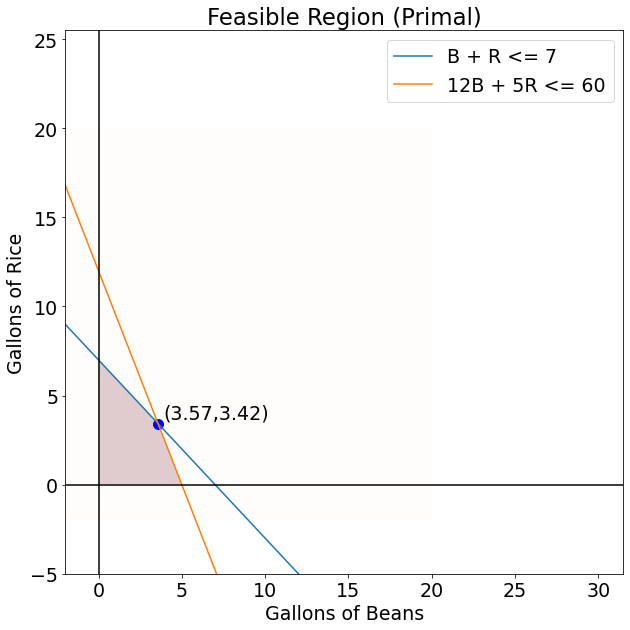
\includegraphics[scale=.33]{feasible_out.png}
            \end{subfigure}%
            ~
            \begin{subfigure}{0.5\textwidth}
                \centering
                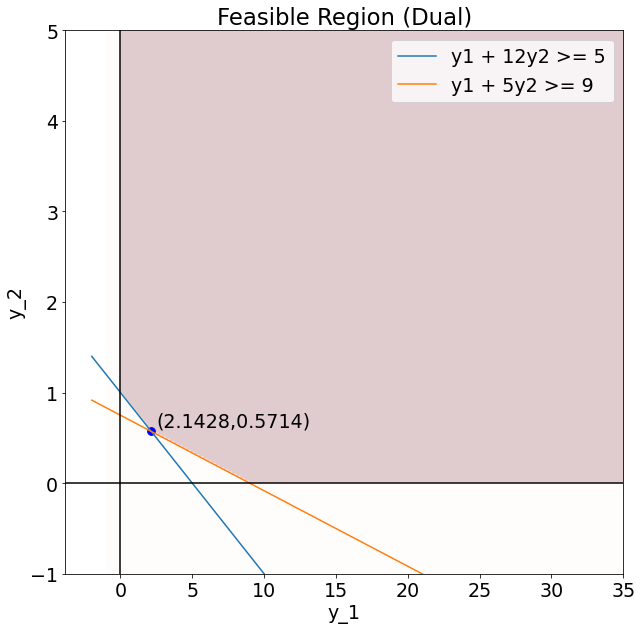
\includegraphics[scale=.33]{dual_out_2.png}
            \end{subfigure}
        \end{figure}

        We can now ask ourselves about complementary slackness and the strong
        duality theorems. We know that strong duality dictates the following...
        \[
            c \cdot x^* = b^T \cdot y^*
        \]
        Such that if the strong duality theorem holds for this optimization
        problem, this will be true. We can test this quickly by taking the
        following
        \[
            c \cdot x^* = 
            \begin{bmatrix} 9   &   5 \end{bmatrix}
            \cdot
            \begin{bmatrix} 3.57   \\   3.42 \end{bmatrix}
            = 49.286
        \]
        And...
        \[
            b^T \cdot y^* =
            \begin{bmatrix} 7   &   60 \end{bmatrix}
            \cdot
            \begin{bmatrix} 2.143  \\  0.571 \end{bmatrix}
            = 49.286
        \]
        So we can see that the strong duality theorem holds. We now care to
        test if complementary slackness upholds in this context. To test this,
        we can use complementary slackness theorem which states the following
        must be true.
        \[
            (b-Ax)^T \cdot y = 0 = (y^TA-c) \cdot x 
        \]
        This can be tested, and by quickly plugging these into Numpy, we get
        the result that the complementary slackness theorem is upheld (up to
        computational error).

        The dual price $y_1 = 2.143$ is associated with the primal
        constraint regarding the gallons of food (or $B+R \leq 7$) and the dual
        price $y_2 = 0.571$ is associated with the constraint regarding the
        unit price of nutritional days of food (or $12B + 5R \leq 60$).
        
        \newpage

    \item Suppose you increase the barrel size to accomodate $c$ gallons of
        food. Does the dual price for the modified constraint provide an
        accurate prediction of the increase in the primal objective function?
        Answer for $c = 1, 2, 4, 6$. \\
        
        We know the dual price variable is given by $y^* =
        [\;2.143,\;0.571\;]$, which, via the dual price lemma, means that we
        should expect that for every one gallon we increase our barrell size
        by, our primal objective function value should increase in
        approximate accordance with the value of the dual price variable. We
        can test this, by running the linear program against the values $7 + c$
        for all given $c$. The results are given in the following table.
        \begin{center}
            \begin{tabular}{|| c | c | c ||}
                \hline
                \multicolumn{3}{|| c ||}{Dual price predictions} \\
                \hline
                7 + c   &   Primal Obj. Func. Val   &   Difference   \\
                \hline \hline

                c = 0   &   49.29   &   N/A     \\
                c = 1   &   51.42   &   2.13    \\
                c = 2   &   53.57   &   2.15    \\
                c = 4   &   57.85   &   4.28    \\
                c = 6   &   60.00   &   2.15    \\

                \hline
            \end{tabular}
        \end{center} 

        We can see here that the dual variable is actually a rather accurate
        predictor of just how the primal objective function will increase. This
        is, of course, until the difference begins to become larger, in which
        case it seems to become less accurate. This is largely due to the fact
        that, up until the value of 13 for the gallons of food, the dual price
        remained the same, but after this value, it changes. I am not entirely
        certain why this is the case. So for now, it is simply an observed
        behavior.

\end{enumerate}

\item You're at a yard sale and have spied four crates of goods. Crates A, B,
    C, and D. They are worth \$5000, \$600, \$3500, and \$6000 respectively,
    but you can buy them from the yard sale for \$24, \$76, \$43, \$754. You
    have \$800, and can carry 85 pounds. The crates weigh 75.5, 2.7, 3.3, and
    6.7 pounds (A, B, C, and D). Given that there is only one of each crate,
    you wish to maximize your turn around profit.

    \begin{enumerate}
    \item Write the above as an integer linear program.

        To start, we should identify our objective function, and our
        constraints. We know that what we wish to maximize is our profit, which
        can be regarded as our revenue minus our costs (ie $P(A, B, C, D) =
        R(A, B, C, D) - q(A, B, C, D)$). This can be written as follows.
        \[
            c = [\; 4976,\; 524,\; 3457,\; 5264\; ]
        \]
        We also know that we are constrained in weight and buying power by the
        following relations:
        \begin{align*}
            24A + 76B + 43C + 754D &\leq 800 \\
            75.5A + 2.7B + 3.3C + 6.7D &\leq 85
        \end{align*}
        We also know that for each crate, we can only by one of them. So we
        define a constraint matrix A as follows.
        \[
            A = \begin{bmatrix}
                    24      &       76      &       43      &       754 \\
                    75.5    &       2.7     &       3.3     &       6.7 \\
                    1       &       0       &       0       &       0   \\
                    0       &       1       &       0       &       0   \\
                    0       &       0       &       1       &       0   \\
                    0       &       0       &       0       &       1   \\
                \end{bmatrix},\;\;\;
            b = \begin{bmatrix}
                    800 \\  85  \\  1  \\  1  \\  1  \\  1
                \end{bmatrix}
        \]
        Right off the bat, we can attempt to run this as a standard, primal
        linear program and we will see that we get $x^* =
        [\;.9908,\;0,\;1,\;.9723\;]$. To make this an integer linear
        programming problem, we must take into account that A, B, C, and D can
        ONLY be 1 or 0 and no value inbetween. In this case, that means if the
        solution to the integer linear programming problem is $x^i$, then $x^i
        \geq [\;1\;0\;1\;1\;] \longrightarrow {x^i }$ is infeasible. We can now
        use the branch and bound algorithm to find the optimal value.

    \item Execute Branch and Bound
        We can execute the entire branch and bound algorithm based on the
        constraints given and that we already have two integer values (in the
        actual example I work out, I treat B as a non-integer because I could
        not determine whether or not to account to computational error at this
        order of magnitude). We prune any node whose value change violated the
        constraints, and we prune any integer value that is not maximal. If we
        do the whole problem out and put the results into a graph, we get the
        following.

    \item Draw the branch and bound tree for the solution

        I drew the tree on the following page so it could be blown up to a
        decent enough proportion. In the problem, I assumed that we only had
        one integer solution, as most of the others were only approximately 0
        or 1, and thus I branched on every variable save for $D$. The final
        solution came out to be one of crate $C$ and one of crate $D$, which
        totalled \$8557.59.

        \begin{figure}[h]
            \centering
            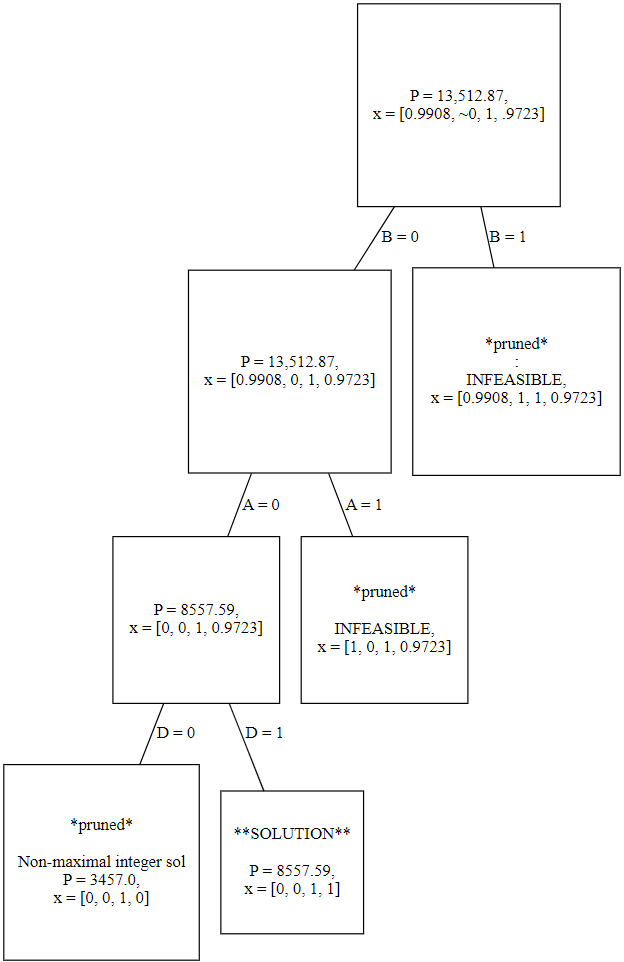
\includegraphics[scale=.9]{unknown.png}
        \end{figure}





    \end{enumerate}


\end{enumerate}
\end{document}
